\documentclass[10pt]{article}
\usepackage{luatexja-fontspec}
\usepackage[a4paper, margin=1in]{geometry}
\usepackage{tikz}
\usetikzlibrary{calc,patterns,angles,quotes}
\usepackage{booktabs}
\usepackage[skins]{tcolorbox}
\usepackage{mathandphy}
\usepackage{graphicx}
\usepackage{float} %设置图片浮动位置的宏包
\usepackage{subfigure} %插入多图时用子图显示的宏包
\usepackage{multicol}

\begin{document}
\noindent 電磁気学\ 第一回 \hfill Homework \#\\
Satanya@張睿 (10/4)

\hrulefill

\begin{problem}
求解電偶極子軸線和中垂面上的電場強度
%fig 1
\begin{figure}[H]
    \centering %图片居中
    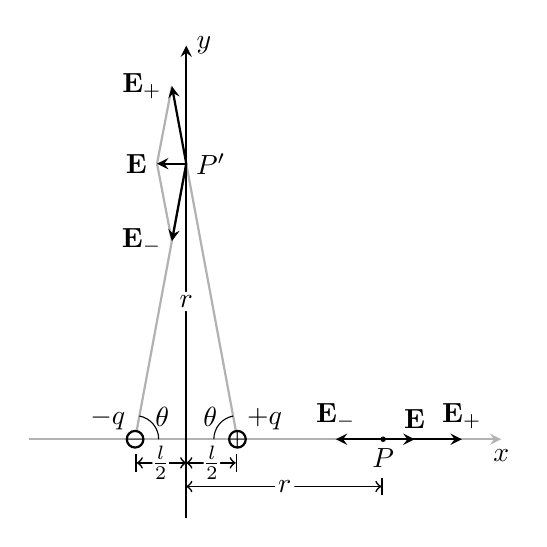
\begin{tikzpicture}
        \coordinate (o) at (0,0);
        \coordinate[label=above left:$-q$] (fu) at (-0.65, 0) {};
        \coordinate[label=above right:$+q$] (zh) at (0.65, 0) {};
        \coordinate[label=right:$P'$] (P') at (0, 3.5) {};
        \coordinate[label=below:$P$] (P) at (2.5, 0) {};

        \draw[thick, black!30] (P') -- (fu);
        \draw[thick, black!30] (P') -- (zh);

        \draw[-stealth, thick, black!30] (-2,0)--(4,0) node[below, black] {$x$};
        \draw[-stealth, thick] (0,-1)--(0,5) node[right] {$y$};

        \fill[fill=white, draw=black, thick] (fu) node{$-$} circle [radius = 3pt];
        \fill[fill=white, draw=black, thick] (zh) node{$+$} circle [radius = 3pt];

        \fill (P) circle[radius=1pt];

        \draw[thick, black!30] ($(P')!-1cm!(zh)$) -- (-0.3714cm, 3.5);
        \draw[thick, black!30] ($(P')!1cm!(fu)$) -- (-0.3714cm, 3.5);

        \pic [draw, -, "$\theta$", angle radius=0.3cm, angle eccentricity=1.5] {angle = o--fu--P'};
        \pic [draw, -, "$\theta$", angle radius=0.3cm, angle eccentricity=1.5] {angle = P'--zh--o};

        \draw[thick, -stealth] (P') -- ($(P')!1cm!(fu)$) node[left] {$\mathbf{E}_-$};
        \draw[thick, -stealth] (P') -- ($(P')!-1cm!(zh)$) node[left] {$\mathbf{E}_+$};
        \draw[thick, -stealth] (P') -- +(180: 0.3714cm) node[left] {$\mathbf{E}$};

        \draw[thick, -stealth]  (P) -- +(0: 1cm) node[above] {$\mathbf{E}_+$};
        \draw[thick, -stealth]  (P) -- +(180: 0.6cm) node[above] {$\mathbf{E}_-$};
        \draw[thick, -stealth]  (P) -- +(0: 0.4cm) node[above] {$\mathbf{E}$};

        \draw[|<->, semithick] (-0.65, -0.3) -- (0, -0.3);
        \draw[<->|, semithick] (0, -0.3) -- (0.65, -0.3);
        \draw[<->|, semithick] (0, -0.6) -- (2.5, -0.6);
        \fill[fill=white] (-0.325, -0.3) node{$\frac{l}{2}$} circle [radius = 3pt];
        \fill[fill=white] (0.325, -0.3) node{$\frac{l}{2}$} circle [radius = 3pt];

        \fill[fill=white] (1.25, -0.6) node{$r$} circle [radius = 3.5pt];
        \fill[fill=white] (0, 1.75) node{$r$} circle [radius = 3.5pt];
    \end{tikzpicture}
    \caption{電偶極子} %最终文档中希望显示的图片标题
\end{figure}
\end{problem}

\begin{solve}
    設 $(\vu{i},\vu{j},\vu{k})$ 是 $\mathbb{R}^3$ 的標準基.
    \begin{itemize}
        \item[1)]對於延長線上的$P$點
              \begin{align*}
                  \va{E}_+ & = \frac{1}{4\pi\varepsilon_0}\frac{q}{\left(r - \frac{l}{2}\right)^2} \vu{i}  \\
                  \va{E}_- & = \frac{1}{4\pi\varepsilon_0}\frac{-q}{\left(r + \frac{l}{2}\right)^2} \vu{i}
              \end{align*}
              因此
              \begin{align*}
                  \va{E} = \va{E}_+ + \va{E}_-
                   & = \frac{1}{4\pi\varepsilon_0}\left[\frac{q}{\left(r-\frac{l}{2}\right)^2}-\frac{q}{\left(r+\frac{l}{2}\right)^2}\right]\vu{i}      \\
                   & = \frac{q}{4\pi\varepsilon_0r^2}\left[\frac{1}{\left(1-\frac{l}{2r}\right)^2}-\frac{1}{\left(1+\frac{l}{2r}\right)^2}\right]\vu{i} \\
                   & \approx \frac{q}{4\pi\varepsilon_0r^2} \left(1+\frac{l}{r} - 1 + \frac{l}{r}\right) \vu{i}                                         \\
                   & = \frac{2ql}{4\pi\varepsilon_0r^3}\vu{i}
              \end{align*}
              定義 $\va{l} = -l\vu{i}$ 及電偶極距矢量 $\va{p} = q\va{l}$
              $$
                  \va{E} \approx -\frac{1}{4\pi\varepsilon_0}\frac{2\va{p}}{r^3}
              $$

        \item[2)]對於中軸線上的$P'$點
              \begin{align*}
                  \va{E}_+ & = \frac{1}{4\pi\varepsilon_0}\frac{q}{r^2 + \frac{l^2}{4}}(-\cos \theta \vu{i} + \sin \theta \vu{j}) \\
                  \va{E}_- & = \frac{1}{4\pi\varepsilon_0}\frac{-q}{r^2 + \frac{l^2}{4}}(\cos \theta \vu{i} + \sin \theta \vu{j})
              \end{align*}
              所以
              \begin{align*}
                  \va{E} = \va{E}_{+} + \va{E}_{-} & = -2\frac{1}{4\pi\varepsilon_0}\frac{q}{r^2 + \frac{l^2}{4}}\cos \theta \vu{i}                                   \\
                                                   & = -\frac{1}{2\pi\varepsilon_0}\frac{q}{r^2 + \frac{l^2}{4}}\frac{\frac{l}{2}}{\sqrt{r^2 + \frac{l^2}{4}}} \vu{i} \\
                                                   & = -\frac{1}{4\pi\varepsilon_0}\frac{ql}{\left(r^2 + \frac{l^2}{4}\right)^{3/2}} \vu{i}                           \\
                                                   & = -\frac{1}{4\pi\varepsilon_0}\frac{ql}{r^3\left(1 + \frac{l^2}{4r^2}\right)^{3/2}} \vu{i}
              \end{align*}
              因爲 $r \gg \frac{l}{2}$, $\left(1 + \frac{l^2}{4r^2}\right)^{3/2} \approx 1$, 又可以定義 $\va{l} = -l\vu{i}$ 及電偶極距矢量 $\va{p} = q\va{l}$,
              \begin{equation*}
                  \va{E} \approx \frac{1}{4\pi\varepsilon_0}\frac{\va{p}}{r^3} \qedhere
              \end{equation*}
    \end{itemize}
\end{solve}
\begin{problem}
使用馬克士威方程組(Maxwell's equations)推導光速 $c$.
$$
	\begin{cases}
		 & \nabla \cdot \va{E} = 0                                                       \\
		 & \nabla \cdot \va{B} = 0                                                       \\
		 & \nabla \times \va{E} = -\frac{\partial\va{B}}{\partial t}                     \\
		 & \nabla \times \va{B} = \mu_0\varepsilon_0 \frac{\partial \va{E}} {\partial t}
	\end{cases}
$$
Hint: $\nabla \times (\nabla \times \va{A}) = \nabla(\nabla \cdot \va{A}) - \nabla^2\va{A}$
\end{problem}
\begin{solve}
	\begin{align*}
		\text{与式} & = \lim_{x \to 0} \frac{\frac{1}{2}(1 - x^2)^{-\frac{1}{2}}(-2x) + 3\sin 3x}{e^x - 1}                                                         \\
		            & = \lim_{x \to 0} \frac{\frac{1}{2}(-\frac{1}{2})(1 - x^2)^{-\frac{3}{2}}(-2x)^2 + (-2)[\frac{1}{2}(1 - x^2)^{-\frac{1}{2}}] + 9\cos 3x}{e^x} \\
		            & = 8 \qedhere
	\end{align*}
\end{solve}
\begin{problem}
庫侖定律和高斯定理互相推導過程
\begin{align*}
    \text{庫倫定律:} & \mathbf{E} = \frac{1}{4\pi\varepsilon_0} \frac{q}{r^2} \hat{\mathbf{r}}                                                     \\
    \text{高斯定理:} & \Phi_{E} = \oiint_{\mathbb{S}} \mathbf{E} \cdot \dif \mathbf{S} = \frac{1}{\varepsilon_0} \sum_{i(\mathbb{S}\text{内})} q_i
\end{align*}

\end{problem}

\begin{solve}
    極座標下,對於半徑爲$r$的一球面面元$\dif A$,
    $$\dif A = (r\sin\theta\dif\varphi)(r\dif\theta)$$
    可定義極小立體角爲
    $$\dif\Omega = \frac{\dif A}{r^2} = \sin\theta\dif\theta\dif\varphi$$
    對於更加普遍的有向面元$\dif\va{S} = \dif S\vu{n}$而言, 可推廣立體角定義爲
    $$\dif\Omega  = \frac{(\vu{r}\cdot\vu{n})\dif S}{r^2} = \frac{\vu{r}\cdot\vu{n}}{\left\|\vu{r}\cdot\vu{n}\right\|}\sin\theta\dif\theta\dif\varphi$$
    由立體角的推廣定義,對於任一封閉曲面$\mathbb{S}$所張之立體角也就有所定義了,當頂點在曲面内時, 對於曲面上的任一立體角元$\dif\Omega$,其$\vu{r}$和$\vu{n}$夾角總小於$\pi/2$, 即 $(\vu{r}\cdot\vu{n})/{\left\|\vu{r}\cdot\vu{n}\right\|} \equiv 1$
    $$
        \oiint_\mathbb{S} \dif\Omega = \oiint_\mathbb{S} \sin\theta \dif\theta \dif\varphi = \int_0^\pi \sin\theta \dif\theta \int_0^{2\pi} \dif\varphi = [-cos\theta]_0^{\pi} (2\pi)  = 4\pi
    $$
    當頂點在曲面外時, 對於曲面上的任一立體角元$\dif\Omega$皆存在一個互爲相反數立體角元$\dif\Omega$, 使得積分結果爲$0$
    $$
        \oiint_\mathbb{S} \dif\Omega = 0
    $$
    \begin{itemize}
        \item[1)] 庫倫定律 $\rightarrow$ 高斯定理\\
              電通量$\Phi_E$乃電場在高斯面各處的法向分量的總和.

              \columnseprule=0.4pt
              \begin{multicols}{2}
                  \begin{itemize}
                      \item[a)] $q$在高斯面内的情況
                            \begin{align*}
                                \Phi_E & = \oiint_{\mathbb{S}} \mathbf{E} \cdot \dif \mathbf{S}                                            \\
                                       & = \oiint_{\mathbb{S}} \frac{1}{4\pi\varepsilon_0} \frac{q}{r^2} \hat{\mathbf{r}} \cdot \dif\va{S} \\
                                       & = \oiint_{\mathbb{S}} \frac{q}{4\pi\varepsilon_0} \dif\Omega                                      \\
                                       & = \frac{q}{\varepsilon_0}
                            \end{align*}

                      \item[b)] $q$在高斯面外的情況
                            \begin{align*}
                                \Phi_E & = \oiint_{\mathbb{S}} \mathbf{E} \cdot \dif \mathbf{S}                                            \\
                                       & = \oiint_{\mathbb{S}} \frac{1}{4\pi\varepsilon_0} \frac{q}{r^2} \hat{\mathbf{r}} \cdot \dif\va{S} \\
                                       & = \oiint_{\mathbb{S}} \frac{q}{4\pi\varepsilon_0} \dif\Omega                                      \\
                                       & = 0
                            \end{align*}
                  \end{itemize}
              \end{multicols}


              \begin{itemize}
                  \item[c)] 數個點電荷組成電荷系的情況

                        電荷系可分爲面内和面外兩個部分, 由a)、b)的結論和場強疊加原理得
                        \begin{align*}
                            \Phi_E & = \oiint_{\mathbb{S}}\left(\sum_{i(\mathbb{S}\text{内})}\mathbf{E}_i + \sum_{j(\mathbb{S}\text{外})}\mathbf{E}_j\right)\cdot \dif \mathbf{S}                            \\
                                   & = \sum_{i(\mathbb{S}\text{内})}\oiint_{\mathbb{S}}\mathbf{E}_i\cdot \dif \mathbf{S} + \sum_{j(\mathbb{S}\text{外})}\oiint_{\mathbb{S}}\mathbf{E}_j\cdot \dif \mathbf{S} \\
                                   & = \sum_{i(\mathbb{S}\text{内})}\frac{q_i}{\varepsilon_0} + \sum_{j(\mathbb{S}\text{外})} 0                                                                              \\
                                   & = \frac{1}{\varepsilon_0}\sum_{i(\mathbb{S}\text{内})} q_i                                                                                                              \\
                        \end{align*}
              \end{itemize}


        \item[2)] 高斯定理 $\rightarrow$ 庫倫定律\\
              設一點電荷$q$, 以其爲球心, $r$爲半徑假設球形高斯面, 則有
              $$\oiint_{\mathbb{S}} \va{E} \cdot \dif\va{S} = \frac{q}{\varepsilon_0}$$
              $$\oiint_{\mathbb{S}} \va{E} \cdot \vu{r} \dif S = \frac{q}{\varepsilon_0}$$
              因爲$\va{E}$和$\vu{r}$處處平行, 場強大小在球面上處處相等, 故
              $$\va{E} \cdot \vu{r} \oiint_{\mathbb{S}} \dif S = \frac{q}{\varepsilon_0}$$
              又因爲$\vu{r}^2 = 1$, $\vu{r}$自反, 所以
              \begin{equation*}
                  \va{E} = \frac{\vu{r}}{4\pi r^2}\frac{q}{\varepsilon_0} = \frac{1}{4\pi\varepsilon_0}\frac{q}{r^2}\vu{r} \qedhere
              \end{equation*}
    \end{itemize}
\end{solve}

\newpage
\hrulefill
\begin{table}[!htbp]
    \centering
    \begin{tabular}{lcc}
        \toprule
        符號             & 物理意義   & 單位(MKSA)           \\
        \midrule
        $q$              & 電荷       & $\unit{C}$           \\
        $\va{E}$         & 電場       & $\unit{N/C(或V/m)}$  \\
        $\va{B}$         & 磁場       & $\unit{T}$           \\
        $\Phi_E$         & 電通量     & $\unit{J\cdot m /C}$ \\
        $\Phi_B$         & 磁通量     & $\unit{Wb}$          \\
        $\mathbb{S}$     & 積分曲面   & $\unit{m^2}$         \\
        $\mathbb{L}$     & 積分環路   & $\unit{m}$           \\
        $\dif \va{S}$    & 面元       & $\unit{m^2}$         \\
        $\dif \bm{\ell}$ & 線元       & $\unit{m}$           \\
        $c$              & 光速       & m/s                  \\
        $\varepsilon_0$  & 真空電容率 & $\unit{F/m}$         \\
        $\mu_0$          & 真空磁導率 & $\unit{H/m}$         \\
        \bottomrule
    \end{tabular}
\end{table}

\begin{table}[!htbp]
    \centering
    \begin{tabular}{ccc}
        \toprule
        符號            & 數學意義           \\
        \midrule
        $\nabla \cdot$  & 散度算符           \\
        $\nabla \times$ & 旋度算符           \\
        $\Im$           & 虛部               \\
        $\Re$           & 實部               \\
        $a$             & 純量               \\
        $\va{v}$        & 向量               \\
        $\vu{v}$        & $\va{v}$的單位向量 \\
        $\norm{\va{v}}$ & 範數               \\
        $\mathbb{R}^n$  & $n$維歐幾里得空間  \\
        \bottomrule
    \end{tabular}
\end{table}

\end{document}
